\documentclass[tikz,border=6pt]{standalone}
\usetikzlibrary{arrows.meta,positioning}
\begin{document}
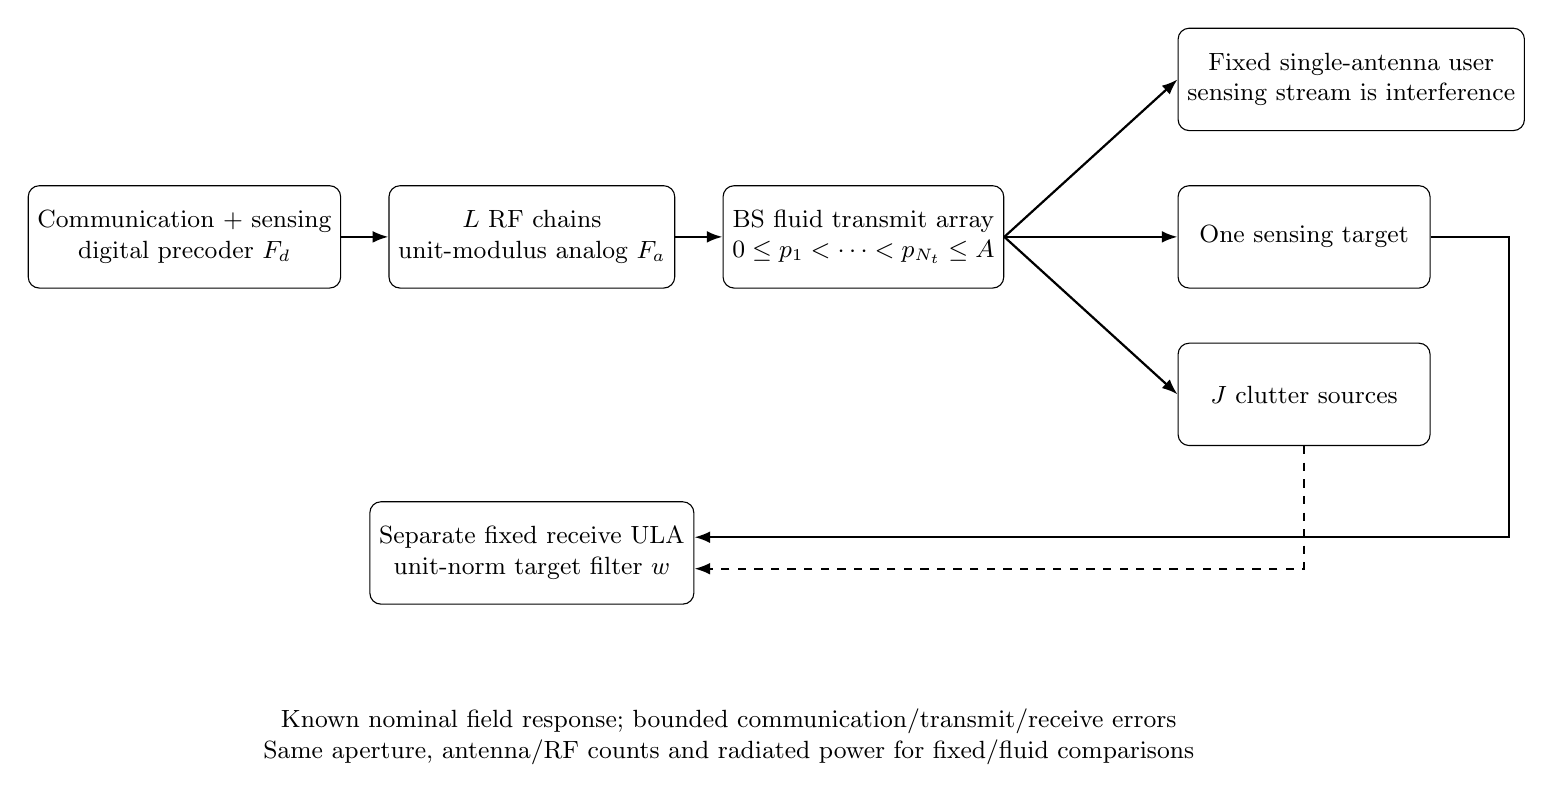
\begin{tikzpicture}[font=\small,arr/.style={-{Latex[length=2mm]},thick},box/.style={draw,rounded corners,align=center,minimum width=32mm,minimum height=13mm}]
\node[box] (bb) {Communication + sensing\\digital precoder $F_d$};
\node[box,right=6mm of bb] (rf) {$L$ RF chains\\unit-modulus analog $F_a$};
\node[box,right=6mm of rf] (tx) {BS fluid transmit array\\$0\le p_1<\cdots<p_{N_t}\le A$};
\draw[arr] (bb)--(rf);\draw[arr] (rf)--(tx);
\node[box,right=22mm of tx,yshift=20mm] (user) {Fixed single-antenna user\\sensing stream is interference};
\node[box,right=22mm of tx] (target) {One sensing target};
\node[box,right=22mm of tx,yshift=-20mm] (clutter) {$J$ clutter sources};
\draw[arr] (tx.east)--(user.west);\draw[arr] (tx.east)--(target.west);\draw[arr] (tx.east)--(clutter.west);
\node[box,below=27mm of rf] (rx) {Separate fixed receive ULA\\unit-norm target filter $w$};
\draw[arr] (target.east) -- ++(10mm,0) |- ([yshift=2mm]rx.east);\draw[arr,dashed] (clutter.south) |- ([yshift=-2mm]rx.east);
\node[below=12mm of rx,xshift=25mm,text width=170mm,align=center] {Known nominal field response; bounded communication/transmit/receive errors\\Same aperture, antenna/RF counts and radiated power for fixed/fluid comparisons};
\end{tikzpicture}
\end{document}
